\input{Header-FSM.tex}

\begin{document}

\begin{page}
\centering
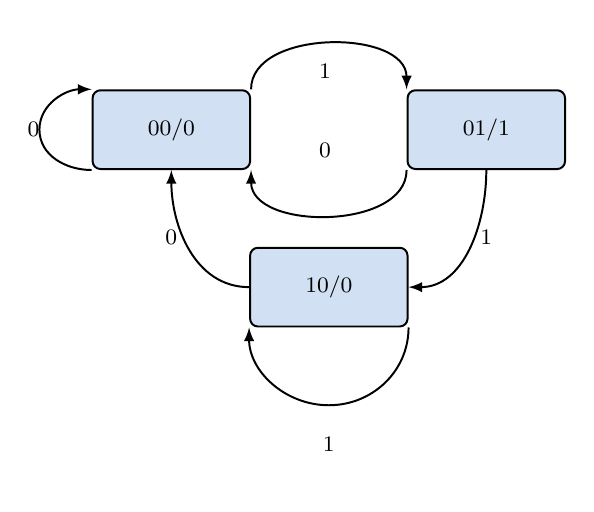
\begin{tikzpicture}

	%DEFINICIONES
	\tikzstyle{every node}=[font=\footnotesize]	
	\tikzstyle{base} = [draw, align=center, line width=0.25mm, fill={rgb,255:red,204; green,255; blue,204}, minimum width=2cm, minimum height=1.25cm]	
	\tikzstyle{blank} = [align=center, inner sep=0pt, outer sep=0pt]	
	\tikzstyle{block} = [draw, rounded corners=0.1cm, align=center, line width=0.25mm, fill={rgb,255:red,209; green,225; blue,243}, minimum width=2cm, minimum height=2cm]	
	\tikzstyle{flecha} = [->, line width=0.25mm, >=latex]
	\tikzstyle{linea} = [line width=0.25mm, >=latex]
	\tikzstyle{meas} = [draw, rectangle, densely dashed, minimum width=0.2cm, minimum height=0.6cm]
	\tikzstyle{circulo} = [circle,fill=black,inner sep=0pt,minimum size=3pt]
	
	%BLOQUES
	\draw(0,0) node[block, minimum height=1cm](1){00/0};
	\draw(4,0) node[block, minimum height=1cm](2){01/1};
	\draw(2,-2) node[block, minimum height=1cm](3){10/0};
	
	\draw(-1.75,0) node[blank, minimum height=1cm](4){0};	%LOOP DEL 1
	\draw(2,-4) node[blank, minimum height=1cm](5){1};	%LOOP DEL 3
	
	%FLECHAS
	\draw [flecha] (1.north east) to[out=90,in=90] (2.north west) node[midway, blank, label=above:$1$, yshift=0.5cm, xshift=1.95cm]{};
	\draw [flecha] (2.south west) to[out=-90,in=-90] (1.south east) node[midway, blank, label=above:$0$, yshift=-0.5cm, xshift=1.95cm]{};
	\draw [flecha] (2.south) to[out=-90,in=0] (3.east) node[midway, blank, label=above:$1$, yshift=-1.6cm, xshift=4cm]{};
	\draw [flecha] (3.west) to[out=180,in=-90] (1.south) node[midway, blank, label=above:$0$, yshift=-1.6cm]{};
	

	\draw [flecha] (1.south west) to[out=180,in=-90] (4.east) to[out=90,in=180] (1.north west);	%LOOP DEL 1	
	\draw [flecha] (3.south east) to[out=-90,in=0] (5.north) to[out=-180,in=-90] (3.south west);	%LOOP DEL 3
\end{tikzpicture}	
\end{page}

\end{document}